\chapter{Apron design}

	\section{Introduction}
	The apron is the area of an airport where the aircraft are parked, unloaded or loaded, refuelled and boarded. It also has to cover the taxiways and the trajectories that air planes have to take in order to get to the principal taxiways or the station zones.  
	
	Another function that the apron has to full-fill is the creation of a service way that will allow all the different services needed by the plane to get to it and the creation of some waiting positions for them that will not obstacle the manoeuvres of the plane. Last but not least, the connection between air-side and land-side is under the responsibility of the apron. 
	
	Before moving into a more detailed explanation of each part that makes the apron, a general view is going to be attached in order to obtain a general idea of what is the apron.
	
	\begin{figure}[H]
		\centering
		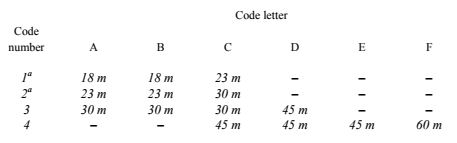
\includegraphics[clip, trim=0cm 0cm 0cm 0cm, width=1\textwidth]{./images/Annex14/RunwayWidth}
		\caption{Runway width according to OACI.} %nom de la figura
		\label{} %per denotar una referencia
	\end{figure}
	
	
	The sections of the apron that will be further explained are the apron taxiways, the aircraft stands, the apron trajectories, service ways and terminal connections. 
	
	\section{Apron taxiways}
	
	\section{Aircraft stands}
		\subsection{General dimensions of aircraft stands}
		\subsection{Dimensions for reference aircraft}
		\subsection{Aircraft stands organization}
			
	\section{Apron trajectories}
	
	\section{Service ways in apron}
	
	\section{Terminal connections}
	